\documentclass[unknownkeysallowed]{beamer}
\usepackage[french,english]{babel}
\usepackage{etex} %solve bugs with listings
\usefonttheme[onlymath]{serif} % rounded shapes for maths
\usepackage[utf8]{inputenc}
\usepackage[T1]{fontenc}% accents (for pdf)
\usepackage{lmodern}
\usepackage{xcolor}
\usepackage{verbatim}
\usepackage{dsfont}
\usepackage[thicklines]{cancel}  % to strike out a text / text rayé
\renewcommand{\CancelColor}{\red}
%
\usepackage{graphicx}
\graphicspath{{images/},{prebuiltimages/},{../../sharedimages/}}

\usepackage{amsmath,amssymb,amsfonts,amscd}

\usepackage{appendixnumberbeamer} % to remove counter for appendix.

\usepackage{multicol}
\usepackage{subcaption}
\usepackage{caption}
% \usepackage{algpseudocode}
\hypersetup{colorlinks,linkcolor=,urlcolor=blue}
\usepackage{latexsym}
\usepackage{fancyhdr} % for page layout
\usepackage{stmaryrd} % for llbracket
% \usepackage{transparent}   % for inkscape transparent style (in conflict with tikz)
\usepackage[absolute,overlay]{textpos} % texpos for special fixed positionning of an image
\usepackage{multirow}
\usepackage{blkarray} % block matrix
\usepackage{xparse,soul} %  strikethrough text (barr\'e), \st

\usepackage{mathtools} % to make boxes inside align env.

%%%%%%%%%%%%%%%%%%%%%%%%%%%%%%%%%%%%%%%%%%%%%%%%%%%%%%%%%%%%%%%%%%%%%%%%%%%%%%%
% Movies
\usepackage{animate}
% \usepackage{movie15} % to be prefered?
% \usepackage{media9}


%\usepackage{amsbsy}
%\usepackage{longtable}
%\renewcommand{\labelitemii}{$\star$}
%\renewcommand{\labelitemi}{$\bullet$}


%%%%%%%%%%%%%%%%%%%%%%%%%%%%%%%%%%%%%%%%%%%%%%%%%%%%%%%%%%%%%%%%%%%%%%%%%%%%%%%
%% citation/footenote in beamer
\usepackage[backend=biber,style=verbose,citetracker=true]{biblatex}
\renewcommand{\footnotesize}{\tiny} % size of footnotes
\renewcommand\multicitedelim{\addsemicolon\space} % for footfullcite to have multiple elements separated by commas.

\renewcommand{\footnoterule}{%
\kern -3pt
\hrule width \textwidth height 1.5pt
\kern 3pt
} % control the line before footnotes


%%%%%%%%%%%%%%%%%%%%%%%%%%%%%%%%%%%%%%%%%%%%%%%%%%%%%%%%%%%%%%%%%%%%%%%%%%%%%%%
% footnote setting: (1), (2), etc.
\usepackage{fnpct}
\AdaptNoteOpt\footcite\multfootcite
\renewcommand*{\thefootnote}{(\arabic{footnote})}

% How to solve problem of comas between footfullcite
\AdaptNoteOpt\footfullcite\multfootfullcite


% Configure style for custom doubled line
\newcommand*{\doublerule}{\hrule width \hsize height 1pt \kern 0.5mm \hrule width \hsize height 2pt}

% Configure function to fill line with doubled line
\newcommand\doublerulefill{\leavevmode\leaders\vbox{\hrule width .1pt\kern1pt\hrule}\hfill\kern0pt }


\newcommand{\mytheorem}[2]{
\doublerulefill\ \framebox{\textbf{#1}}\ \doublerulefill
\vspace{0.1cm}

#2

\doublerulefill
}



%%%%%%%%%%%%%%%%%%%%%%%%%%%%%%%%%%%%%%%%%%%%%%%%%%%%%%%%%%%%%%%%%%%%%%%%%%%%%%%
\beamersetuncovermixins{\opaqueness<1>{15}}{\opaqueness<2->{15}}
%%%%%%%%%%%%%%%%%%%%%%%%%%%%%%%%%%%%%%%%%%%%%%%%%%%%%%%%%%%%%%%%%%%%%%%%%%%%%%%


\mode<presentation>
{
\usetheme{default}
\setbeamertemplate{frametitle}
{
  \begin{centering}
    \textbf{\insertframetitle}
    \par
  \end{centering}
}


\setbeamertemplate{navigation symbols}{}
\setbeamertemplate{bibliography item}[triangle]


%%%%%%%%%%%%%%%%%%%%%%%%%%%%%%%%%%%%%%%%%%%%%%%%%%%%%%%%%%%%%%%%%%%%%%%%%%%%%%%
% Colors

%\usecolortheme[named=macouleur]{structure}
\definecolor{macouleur}{cmyk}{0.2,0.45,0.9,0}%{0.05,0.22,0.89,0}
\definecolor{rltred}{rgb}{0.75,0,0}
\definecolor{oneblue}{rgb}{0,0,0.75}
\definecolor{marron}{rgb}{0.64,0.16,0.16}
\definecolor{forestgreen}{rgb}{0.13,0.54,0.13}
\definecolor{verte}{rgb}{0.13,0.74,0.23}
\definecolor{marronchocolat}{cmyk}{0.15,0.32,0.59,0.19}
\definecolor{parme}{cmyk}{0.05,0.22,0.19,0.5}
\definecolor{rltgreen}{rgb}{0.5,0.01,0.9}%violet
\definecolor{oneblue}{rgb}{0,0,0.75}
\definecolor{purple}{rgb}{0.5,0.5,0.98}
\definecolor{purpleone}{rgb}{0.9,0.5,0.5}
\definecolor{dockerblue}{rgb}{0.11,0.56,0.98}
\definecolor{myblue}{rgb}{0,0.2,0.4}%bien
\definecolor{LightBack}{rgb}{0,0.2,0.4}%{0.2, 0.2,0.4}
\definecolor{freeblue}{rgb}{0.25,0.41,0.88}
\usecolortheme{rose}
}

\newcommand{\tbrown}[1]{\textcolor{brown}{#1}}


\usecolortheme[named=marron]{structure}
\setbeamercolor{block title}{use=structure,fg=white,bg=freeblue}
%\setbeamercolor{math text}{fg=LightBack,bg=macouleur}
\setbeamercolor{block body example}{bg=white}
\beamertemplateroundedblocks
\beamertemplateshadowblocks

%%%%%%%%%%%%%%%%%%%%%%%%%%%%%%%%%%%%%%%%%%%%%%%%%%%%%%%%%%%%%%%%%%%%%%%%%%%%%%%
% To add numbering
\setbeamerfont{page number in head/foot}{size=\tiny}
\setbeamertemplate{footline}[frame number]


%\setbeamercolor{structure}{fg=marron,bg=white}


\newcommand{\citer}[2]{\textcolor{brown}{#1}\nocite{#2}}


% new version for algorithm:

% FRENCH VERSION:
% \usepackage[titlenumbered,ruled,noend,french,onelanguage]{algorithm2e}

% ENGLISH VERSION:
\usepackage[titlenumbered,ruled,noend,onelanguage]{algorithm2e}

\newcommand\mycommfont[1]{\footnotesize\ttfamily\textcolor{blue}{#1}}
\SetCommentSty{mycommfont}
\SetEndCharOfAlgoLine{}
\resetcounteronoverlays{algocf} % for overlay aware algorithms.
\renewcommand{\thealgocf}{} % turn of caption numbering
%% old version for algorithm:
%\usepackage[algo2e]{algorithm2e}% http://csweb.ucc.ie/~dongen/LAF/Algorithms.pdf
%
%\usepackage{float}




%%%%%%%%%%%%%%%%%%%%%%%%%%%%%%%%%%%%%%%%%%%%%%%%%%%%%%%%%%%
%%%%% 	        Algorithmes		             %%%%%
%%%%%%%%%%%%%%%%%%%%%%%%%%%%%%%%%%%%%%%%%%%%%%%%%%%%%%%%%%%

\usepackage{fancyvrb}                  % for fancy verbatim
\usepackage{textcomp}
\usepackage[space=true]{accsupp}
% requires the latest version of package accsupp
\newcommand{\copyablespace}{
    \BeginAccSupp{method=hex,unicode,ActualText=00A0}
\ %
    \EndAccSupp{}
}
\usepackage[procnames]{listings}
\lstset{%
language   = Python,%
% basicstyle = \ttfamily\setstretch{1},%
columns    = fullflexible,%
keywordstyle=\color{javared},
firstnumber=100,
frame=shadowbox,
showstringspaces=false,
morekeywords={import,from,class,def,for,while,if,is,in,elif,
else,not,and,or,print,break,continue,return,True,False,None,access,
as,del,except,exec,finally,global,import,lambda,pass,print,raise,try,assert},
keywordstyle={\color{javared}\bfseries},
commentstyle=\color{javagreen}, %vsomb_col white comments
morecomment=[s][\color{javagreen}]{"""}{"""},
upquote=true,
%% style for number
numbers=none,
resetmargins=true,
xleftmargin=10pt,
linewidth= \linewidth,
numberstyle=\tiny,
stepnumber=1,
numbersep=8pt, %
frame=shadowbox,
rulesepcolor=\color{black},
procnamekeys={def,class},
procnamestyle=\color{oneblue}\textbf,
literate={*}{{\char42}}1
         {-}{{\char45}}1
         {\ }{{\copyablespace}}1
}

\lstnewenvironment{Exemplecode}{}{}


\newenvironment{Framecode}[1]
{\begin{frame}[fragile, environment=Framecode]{#1}}
{\end{frame}}


\definecolor{javared}{rgb}{0.6,0,0} % for strings
\definecolor{javagreen}{rgb}{0.25,0.5,0.35} % comments
\definecolor{javapurple}{rgb}{0.5,0,0.35} % keywords
\definecolor{javadocblue}{rgb}{0.25,0.35,0.75} % javadoc
\definecolor{marron}{rgb}{0.64,0.16,0.16}
\definecolor{orange_js}{RGB}{230,159,0}

\newcommand{\mybold}[1]{\textcolor{marron}{\textbf{#1}}}
\newcommand{\cRm}[1]{\textsc{\romannumeral #1}}


\AtBeginDocument{\setlength\abovedisplayskip{0pt}}% remove top align blanks

\input{shortcuts_js}
%\usepackage{./OrganizationFiles/tex/sty/shortcuts_js}
\usepackage{csquotes}

\graphicspath{{./images/}}

\addbibresource{Bibliographie.bib}
\usepackage{enumerate}
\usepackage{amsmath}
\begin{document}


%%%%%%%%%%%%%%%%%%%%%%%%%%%%%%%%%%%%%%%%%%%%%%%%%%%%%%%%%%%%%%%%%%%%%%%%%%%%%%%
%%%%%%%%%%%%%%%%%%%%%%             Headers               %%%%%%%%%%%%%%%%%%%%%%
%%%%%%%%%%%%%%%%%%%%%%%%%%%%%%%%%%%%%%%%%%%%%%%%%%%%%%%%%%%%%%%%%%%%%%%%%%%%%%%



%%%%%%%%%%%%%%%%%%%%%%%%%%%%%%%%%%%%%%%%%%%%%%%%%%%%%%%%%%%%%%%%%%%%%%%%%%%%%%%
\begin{frame}[noframenumbering]
\thispagestyle{empty}
\bigskip
\bigskip
\begin{center}{
\LARGE\color{marron}
\textbf{HMMA 307 : Advanced Linear Modeling}
\textbf{ }\\
\vspace{0.5cm}
}

\color{marron}
\textbf{Chapter 5 : Random Effects Models}
\end{center}

\vspace{0.5cm}

\begin{center}
\textbf{ISKOUNEN SELENA \ AMAHJOUR WALID \ RUDOLF RÖMISCH } \\
\vspace{0.1cm}
\url{https://github.com/selenaiskounen/CA-HMMA307}\\
\vspace{0.5cm}
Université de Montpellier \\
\end{center}

\centering
\includegraphics[width=0.13\textwidth]{Logo.pdf}
\end{frame}

\begin{frame}{Overview} 
	\tableofcontents
\end{frame}

\section{Random Effect Models}
\begin{frame}{Motivation}
We consider cases where we get random samples from large populations. 
Since the goal is to make statements about properties of whole populations and not about observed individuals, it is rather natural to assume random samples. 
Now we elaborate an example with machines. We assume that we assess the quality of produced samples from some machines.

\end{frame}

\subsection{One-Way ANOVA}
\begin{frame}{One-Way ANOVA: Model}
Our model:

$$
Y_{ij} = \mu + \alpha_i + \epsilon_{ij}
$$
Here we have the following variables and assumptions:
\begin{itemize}
    \item $Y_{ij}$ as the quality of the j-th sample on the i-th machine 
    \item $\mu$ as the global mean
    \item $\alpha_i$ i.i.d.  
    $\sim \mathcal{N}(0,\sigma^2_{\alpha})$ as the effect of the i-th machine
    \item $\epsilon_{ij}$ i.i.d. $\sim \mathcal{N}(0,\sigma^2)$ as the error term for the j-th sample and the i-th machine
\end{itemize}
\end{frame}

\begin{frame}{Specialty}
    The model has strong similarities with the fixed models. But the $\alpha_i's$ are random variables and not fixed unkown parameters.
    With that change the properties of the model will be strongly influenced.
    \begin{itemize}
        \item We get the new parameter $\sigma^2_{\alpha}$
        \item Our model is also called variance components models since we have now two different variances $\sigma^2_{\alpha}$ and $\sigma^2$
    \end{itemize}
\end{frame}

\begin{frame}{Properties}
    We consider some properties for our model:
    \begin{itemize}
        \item The expected value of $Y_{ij}$ is $E[Y_{ij}]=\mu$, since $E[Y_{ij}] = E[\mu + \alpha_i + \epsilon_{ij}] = E[\mu] + E[\alpha_i] + E[\epsilon_{ij}] = \mu$
        \item The variance is $Var(Y_{ij}) = \sigma^2_{\alpha} +\sigma^2$ since
        
        $Var(Y_{ij}) = E[Y_{ij}^2] - E[Y_{ij}]^2
        = E[\mu^2] + E[\mu \alpha_i] + E[\mu \epsilon_{ij}] + E[\alpha_i \mu] + E[\alpha_i \alpha_i] + E[\alpha_i \epsilon_{ij}] + E[\epsilon_{ij} \mu] + E[\epsilon_{ij}\alpha_i] + E[\epsilon_{ij}\epsilon_{ij}] - \mu^2
        = \mu^2 + \mu \underbrace{E[\alpha_i]}_\text{= 0} + \mu \underbrace{E[\epsilon_{ij}]}_\text{= 0} + \underbrace{E[\alpha_i]}_\text{=0}\mu + E[\alpha_i^2] + \underbrace{E[\alpha_i]}_\text{= 0}\underbrace{E[\epsilon_{ij}]}_\text{= 0} + \underbrace{E[\epsilon_{ij}]}_\text{=0}\mu + \underbrace{E[\epsilon_{ij}]}_\text{=0} \underbrace{E[\alpha_i]}_\text{=0} + E[\epsilon_{ij}^2] - \mu^2 
        = E[\alpha_i^2] + E[\epsilon_{ij}^2]
        = \sigma^2_{\alpha} + \sigma^2$
    \end{itemize}
\end{frame}

\begin{frame}
	For the correlation structure we get:
	\begin{equation*}
	D_{it} =
	\begin{cases}
	\quad 0 & i \neq k\\
	\sigma^2_{\alpha}/(\sigma^2_{\alpha} + \sigma^2) & i = k, j\neq l\\
	\quad 1 & i=k, j=l
	\end{cases}
	\end{equation*}
	
	Here we can see that observations from different machines are uncorrelated (here independent) while observations from the same machine are correlated. \\
	$\sigma^2_{\alpha}/(\sigma^2_{\alpha} + \sigma^2)$ is also called the intraclass correlation (ICC). For $\sigma^2_{\alpha} >> \sigma^2$, the ICC gets "large" what means that observations from the same "group" are very similar to each other.
	
	So values "sharing" the same $"\alpha_i "$ are correlated, while in the fixed effects model all values would be independent (because there the $\alpha_i$ are parameters, that is fixed, unknown quantities).
\end{frame}

\begin{frame}
	Parameter estimation for the variance components $\sigma^2_{\alpha}$ and $\sigma^2$ is typically being done with a technique called restricted maximum likelihood (REML).\\
	It is also possible to use the "classical" maximum-likelihood estimator but REML estimates are less biased. The parameter $\mu$ is estimated with maximum-likelihood assuming that the variances are known. 
\end{frame}
\subsection{More than one Factor}
\begin{frame}
	Now we can extend our model to the two-way ANOVA situation.\\
	As an example we have a manufacturer who is developing a new spectrophometer for medical labs. A critical issue is consistency of measurements from day to day among different machines. The response is the triglyceride level [mg/dl] of a sample.
\end{frame}

\begin{frame}{More than One Factor: Model}
	 We use the model:
	\begin{equation*}
		Y_{ijk} = \mu + \alpha_i + \beta_j + (\alpha \beta)_{ij} + \epsilon_{ij},
	\end{equation*}
	for the random effects we have the usual assumptions
	\begin{itemize}
		\item $Y_{ijk}$ is the triglyceride level of the k-th sample on day i and machine j,
		\item $\alpha_i$ i.i.d.  
		$\sim \mathcal{N}(0,\sigma^2_{\alpha})$ is the random effect of day,
		\item $\beta_j$ i.i.d.  
		$\sim \mathcal{N}(0,\sigma^2_{\beta})$ is the random effect of machine,
		\item $(\alpha \beta)_{ij}$ i.i.d.  
		$\sim \mathcal{N}(0,\sigma^2_{\alpha \beta})$ random interaction term between day and machine.
	\end{itemize}
\end{frame}

\subsection{Nesting}
\begin{frame}{Motivation}
	Now we introduce a new concept. We consider the strength of a chemical paste product which was measured for a total of sixty samples coming from ten randomly selected delivery batches each containing three randomly selected casks. Now we can find a new way of combining factors. Cask one in batch 1 has nothing to do with cask one in batch two and so on. The "1" of cask has a different meaning for every batch. Hence, cask and batch are not crossed. We say cask is nested in batch.\\
	The battch effect does not seem to be very pronounced. On the other side, casks within the same batch can be substantially different. Let us now model this with appropriate random effects.
\end{frame}


\begin{frame}{Nesting: Model}
	We can use the model:
	\begin{equation*}
		Y_{ijk} = \mu + \alpha_i + \beta_{j(i)} + \epsilon_{k(ij)}.
	\end{equation*}
	\begin{itemize}
		\item $Y_{ijk}$ is the strength of the k-th sample of cask j in batch i,
		\item $\alpha_i$ i.i.d.  
		$\sim \mathcal{N}(0,\sigma^2_{\alpha})$ is the (random) effect of batch,
		\item $\beta_{j(i)}$ i.i.d.  
		$\sim \mathcal{N}(0,\sigma^2_{\beta})$ is the (random) effect of cask within batch,
		\item $\epsilon_{k(ij)}$ i.i.d.  
		$\sim \mathcal{N}(0,\sigma^2)$ is the error term.
	\end{itemize}
	Here we can see the special notation for $\beta_{j(i)}$ and $\epsilon_{k(ij)}$ which emphasizes that cask is nested in batch.
\end{frame}

\section{Mixed Effects Models}
\begin{frame}{Mixed Effects Models}
	In reality there can be encounters with models which contain both random and fixed effects. \\ We call them mixed effects models.\\
	To model this new concept we consider two examples. One is Data on an experiment to compare three brands of machines used in an industrial process. The other one is about two groups of raters who rated four different cheese types. Every rater got to eat two samples from the same cheese type in random order.
\end{frame}

\begin{frame}{Machine Model}
	
	In this model we assume that there is a population effect, where each worker is allowed to have its own (random) deviation.
	\begin{equation*}
		Y_{ijk} = \mu + \alpha_i + \beta_j + (\alpha \beta)_{ij} + \epsilon_{ijk},
	\end{equation*}
	
	\begin{itemize}
		\item $Y_{ijk}$ is the k-th productivity score of worker j on machine i,
		\item $\alpha_i$ is this thime the fixed effect of machine i (with a side constraint),
		\item $\beta_j$ i.i.d. $\sim \mathcal{N}(0,\sigma^2_{\beta})$ is the random effect of worker j,
		\item $(\alpha \beta)_{ij}$ i.i.d. $\sim \mathcal{N}(0,\sigma^2_{\alpha \beta})$ is the corresponding (random) interaction,
		\item $\epsilon_{ijk}$ i.i.d. $\sim \mathcal{N}(0,\sigma^2)$ is the error term.
	\end{itemize}
	

\end{frame}

\begin{frame}{Interpretation}
	Here we have a special situation. The "average" (over the whole population) productivity "profile" iwth respect to the different machines is given by the fixed effect $\alpha_i$. The (random) deviation of an individual worker consists of a general shift $\beta_j$ (worker specific general productivity level) and a worker specific "preference" $(\alpha \beta)_{ij}$ with respect to the machines.
\end{frame}

\begin{frame}{Cheese Model}
	For the cheese type example we have the following model:
	\begin{equation*}
		Y_{ijk} = \mu + \alpha_i + \beta_j + (\alpha \beta)_{ij} +\delta_{k(i)} + (\beta \delta)_{jk(i)} + \epsilon_{ijkl},
	\end{equation*}
	where
	\begin{itemize}
		\item $\alpha_i$ is the (fixed) effect of background,
		\item $\beta_j$ is the (fixed) effect of cheese type,
		\item $(\alpha \beta)_{ij}$ is the corresponding interaction (fixed effect),
		\item $\delta_{k(i)}$ is the random effect of rater ("general cheese liking level of rater $k(i)$)"
		\item $(\beta \delta)_{jk(i)}$ is the (random) interaction of rater and cheese type ("specific cheese type preference of rater $k(i)$")
	\end{itemize}
\end{frame}

\begin{frame}{Interpretation}
	In this example we have an "average" (over the whole population) preference "profile" with respecht to the different cheese types but every rater can have its own random deviation of this "profile". This deviation consists of a general shift $\delta_{k(i)}$ (general cheese liking of a rater) and a rater specific preference $(\beta \delta)_{jk(i)}$ with respect  to the cheese types.
\end{frame}

\begin{frame}{Example: Rates of O3 in Occitania}

The goal of this data analysis is to find out if there is a significant difference in O3 levels between Montpellier, Toulouse, Perpignan and Albi. 

\vspace{0.2cm}

Consider the following notations:
\begin{itemize}
\item{$\mu_m$ = mean of O3 rate in Montpellier.}
\item{$\mu_t$ = mean of O3 rate in Toulouse}
\item{$\mu_p$ = mean of O3 rate in Perpignan}
\item{$\mu_a$ = mean of O3 rate in Albi}
\end{itemize}

\vspace{0.2cm}

In this case, we are going to do an ANOVA to test:
$H_0:\mu_m=\mu_t=\mu_p=\mu_a$ VS $H_1:\mu_m \neq \mu_t \neq \mu_p \neq \mu_a$
\end{frame}

\begin{frame}{Example: Rates of O3 in Occitania}

We start by doing a violin plot to compare the number of evaluation of the level of O3 in each city. 
\begin{figure}
    \centering
    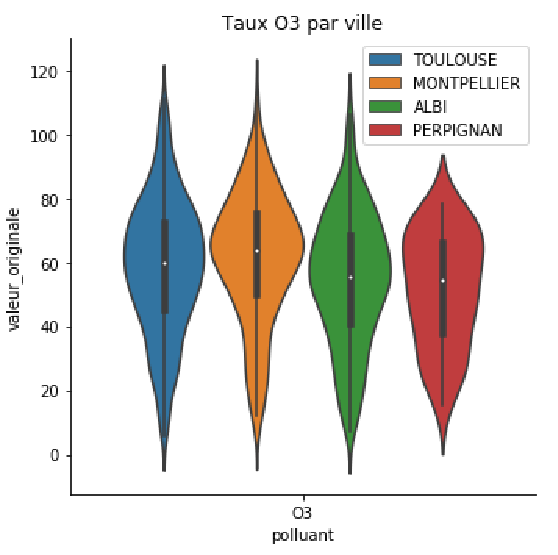
\includegraphics[width=5cm]{carplot.PNG}
    \caption{Violin plot to show the difference between the number of evaluation of 03 in ech city}
    \label{fig:my_label}
\end{figure}
\end{frame}

\begin{frame}{Example: Rates of O3 in Occitania}

As we can see, there's not a significant difference of the number of evaluation of 03 between each city.

Now, we are going make a prognosis on the result of the test using a boxplot.

\begin{figure}
    \centering
    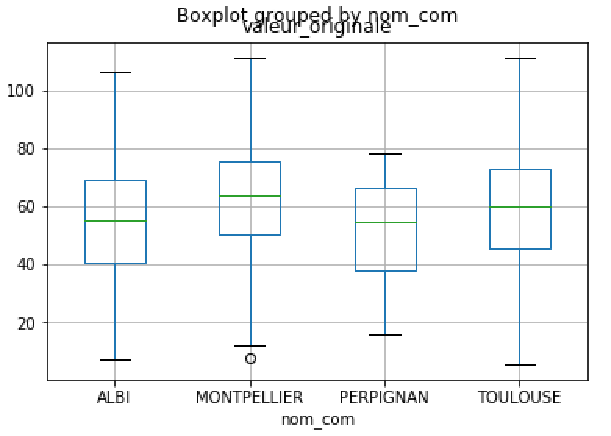
\includegraphics[width=5cm]{boxplot.PNG}
    \caption{ Boxplot of O3 rates in each city}
    \label{fig:my_label}
\end{figure}
 
 We can prognosis that we will reject $H_0$   
\end{frame}

\begin{frame}{Example: Rates of O3 in Occitania}
Now we are going to do the ANOVA to make sure of our prognosis
\begin{figure}
    \centering
    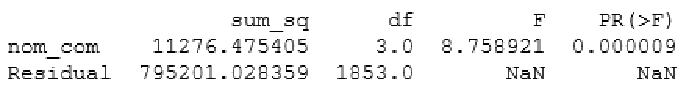
\includegraphics[width=8cm]{resultat.PNG}
    \caption{Results of the ANOVA}
    \label{fig:my_label}
\end{figure}
We obtain F=8.75 > 0.000009, so we will reject $H_0$ and we can say that the levels of 03 differs from one city to another.
\end{frame}








\end{document}